\documentclass[10pt]{article}
\usepackage{amsmath,amsfonts}
\usepackage{graphicx}
\usepackage{float}
% \usepackage{subfig}
\usepackage{subcaption}
\usepackage{epsfig}
\usepackage{color}
\usepackage{algorithm}
\usepackage{algpseudocode}
%---------------------------------------------------------------------------
%Tomo USER DEFINED MACROS

%Response to review macros
\newcommand{\bfc}[1]{{\bf \underline{Response:} }\textnormal{#1}}
\usepackage{color}
% \definecolor{gray}{rgb}{0.5,0.5,0.5}

%%% The following commands are for a marked up version 2, comment for markedup
 % \newcommand{\addone}[1]{\textcolor{violet}{#1}}
 %  \newcommand{\changeone}[1]{\textcolor{red}{#1}}
 %  \newcommand{\doneone}[2][]{\todo[#1]{#2}}
%%% unmarkedup
  \newcommand{\addone}[1]{#1}
  \newcommand{\changeone}[1]{#1}
  \newcommand{\doneone}[2][]{}
%%% The following commands are for an unmarked up version 1, comment for markedup
\newcommand{\added}[1]{#1}
\newcommand{\changed}[1]{#1}
\newcommand{\removed}[1]{}
\newcommand{\done}[2][]{}
\newcommand{\mdone}[1]{}


%Paper body notation
\newcommand{\R}{\mathbb{R}} % reals
\newcommand{\cE}{{\mathcal{E}}} % This will be the set of elements
\newcommand{\cV}{{\mathcal{V}}} % This will be the set of voxels
\newcommand{\cN}{{\mathcal{N}}} % This will be the non-binding set
\newcommand{\cI}{{\mathcal{I}}} % This will be the set of energy channels
\newcommand{\mcT}{{\mathcal{T}}} % This will be the set of energy channels
\newcommand{\cU}{{\mathcal{U}}} % This will be the set of upstream voxels
\newcommand{\cA}{\mathcal{A}} % Active set
\newcommand{\I}[1]{\mathbb{I}_{#1}} % The indicator function
\newcommand{\ones}{\mathbf{1}} % Vector ones
\newcommand{\At}{  A^{E,\theta,\tau}} % Attenuation array
\newcommand{\A}{ {\bf A}} % Attenuation array
\newcommand{\bd}{ {\bf d}} 
\newcommand{\bx}{ {\bf x}} 
\newcommand{\Fl}{\pmb{\mathbf{\rho}}} % Fluorescence emitted array
\newcommand{\Le}{{\bf L}} % length array
\newcommand{\m}{{\bf m}} % M
\newcommand{\cW}{{\mathcal{W}}}
\newcommand{\bcW}{\pmb{\mathbf{\cW}}}
\newcommand{\X}{{\bf X}}
\newcommand{\bc}{{\bf c}}
\newcommand{\byi}{{\bf y_i}}
\newcommand{\bmi}{{\bf m_i}}
\newcommand{\Y}{{\bf Y}}
\newcommand{\ds}{{\displaystyle}}
\newcommand{\argmin}{\operatornamewithlimits{argmin}}
\newcommand{\MD}[1]{{\bf D}_{\theta,\tau}^\mathit{#1}}  % experimental
\newcommand{\MDRi}{D_{\theta,\tau,\iota}^\mathit{R}}  % experimental
\newcommand{\D}[1]{{\bf D}^\mathit{#1}}  % experimental
% data XRF
\newcommand{\MDT}{D_{\theta,\tau}^\mathit{T}}  % experimental data XRF
\newcommand{\tMD}[1]{\pmb{\mathbf{\tilde{D}}}_{\theta,\tau}^\mathit{#1}}  %
% experimental data

\newcommand{\FM}[1]{{\bf F}_{\theta,\tau}^\mathit{#1}} % forward model
\newcommand{\FMRi}{F_{\theta,\tau,\iota}^\mathit{R}} % forward model
% for XRF
\newcommand{\FMT}[1]{{#1}_{\theta,\tau}^\mathit{T}}% forward model for XRT
\newcommand{\J}[1]{{\bf J}^\mathit{#1}} % forward model for XRF


%% macros from CVT
\def \ds          {\displaystyle}
\def \rmd         {{\rm d}}
\def \be          {{\bf e}}
\def \bF          {{\bf F}}
\def \bI          {{\bf I}}
\def \bn          {{\bf n}}
\def \bff         {{\bf f}}
\def \bdf         {{\bf df}}
\def \bdT         {{\bf dT}}
\def \bT          {{\bf T}}
\def \cT          {{\cal T}}
\def \bU          {{\bf U}}
\def \bu          {{\bf u}}
\def \bv          {{\bf v}}
\def \bV          {{\bf V}}
\def \bX          {{\bf X}}
\def \by          {{\bf y}}
\def \bY          {{\bf Y}}
\def \bz          {{\bf z}}
\def \bZ          {{\bf Z}}
\def \bW          {{\bf W}}
\def \bZt         {{\bf \widetilde Z}}
\def \bzi         {{\bz}_i}
\def \bzs         {{\bz}^*}
\def \bzis        {{\bz}_i^*}
\def \bzin        {\{\bzi\}_{i=1}^k}
\def \cf          {{\cal F}}
\def \cg          {{\cal G}}
\def \ch          {{\cal H}}
\def \vi          {{V_i}}
\def \vin         {\{\vi\}_{i=1}^k}
\def \Babs        {{\Big|}}
\def \Bl          {{\Big(}}
\def \Br          {{\Big)}}
\def \Bleft       {{\Big[}}
\def \Bright      {{\Big]}}
\def \p           {\partial}
\def \N           {{\mathbb N}}
\def\y            {{\bf y}}
\def \tN          {{\widetilde{N}}}
\def \tD          {{\widetilde{D}}}

\def \proofnote #1{\footnote{{\bf Note: #1}}}
\def \norm      #1{\left\|\,#1\,\right\|}
\def \set       #1{\left\{\,#1\,\right\}}
\def \tr          {^T}
\def \IhH         {I_h^H}
\def \IhHb        {{\hat I}_h^H}
\def \IHh         {I_H^h}
\def \vbar        {\bar v}
\def \zhbar       {\bar z_h}
\def \zHbar       {\bar z_H}
\def \zhplus      {z_h^+}
\def \zHplus      {z_H^+}

\newcommand{\C}{{\bf C}}
\newcommand{\bmu}{\mathbf{\pmb{\mu}}} % This is for voxel attenuation
\newcommand{\lmu}{\tilde{\mu}}
\newcommand{\cbmu}{{\textcolor{red}{\bmu^E}}}
\newcommand{\blambda}{\pmb{\mathbf{\lambda}}}
\renewcommand{\theequation}{\thesection.\arabic{equation}}

\newtheorem{alg}{Algorithm}[section]
\newtheorem{thm}{Theorem}[section]
\newtheorem{lem}[thm]{Lemma}
\newtheorem{cor}[thm]{Corollary}
\newtheorem{pro}{Proposition}[section]
\newtheorem{defn}{Definition}[section]
\newtheorem{asp}{Assumption}[section]
\newtheorem{rmk}{Remark}[section]
\newtheorem{exmp}{Example}[section]

\newcommand{\SNote}[1]           % For Stefan's margin notes
{\textcolor{blue}{#1}\marginpar{\textcolor{blue}{SW $\longleftarrow$}}}
\newcommand{\cF}{\mathcal{F}}

\title{Extended Abstract: Hierarchical Data Analysis}
\author{Wendy Di, Stefan Wild}
\date{\today}
\begin{document}
  \maketitle 

 \section{Notations}
 {\bf Goal:} Given a halo with $N_p$ particles, find its MBP.
 \begin{itemize}
   \item $D$: dimension of the space, $D=2$ for now
   \item $\X=[X_i]\in \mathbb{R}^{N_p\times 2}$: collection of particles
   \item $\m=[m_i]\in \mathbb{R}^{N_p}$: collection of each particle's mass, normally $m_i=1, \forall i$
   \item $d(x,y)$: Euclidean distance between points $x$ and $y$
   \item $\bar m \in R$: mass of super-particle as a specific collection of particles.  
   \end{itemize}

 \begin{algorithm}
\caption{Naive}
\label{naive}
\begin{algorithmic}[1]
  \State $\ds MBP=\min_i \ds\sum_{j\neq i}\frac{m_j}{d(X_i,X_j)}$
\end{algorithmic} 
 \end{algorithm}
\begin{figure}[H]
\centering
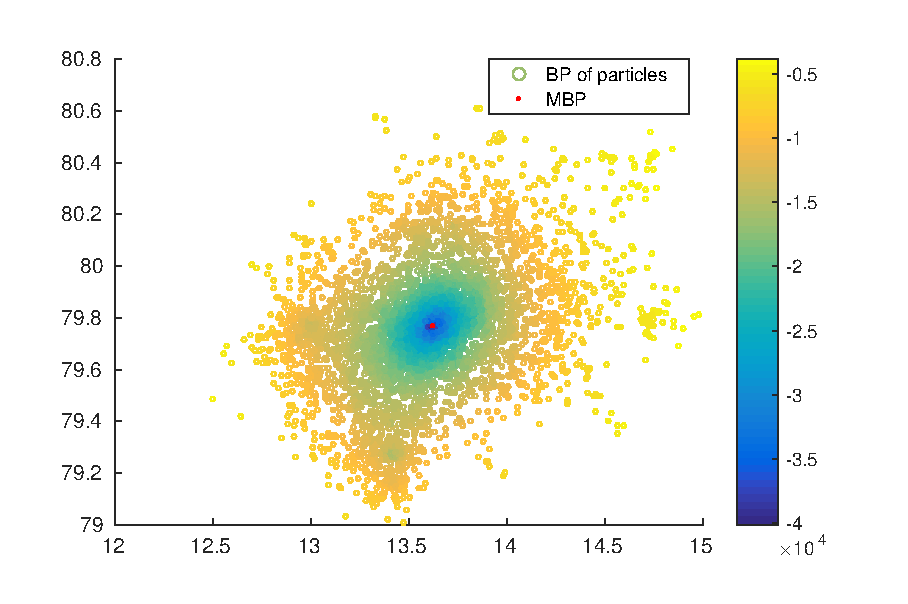
\includegraphics[scale=0.45]{naive}%
\caption{MBP Illustration}
\label{fig:naive}
\end{figure}
 \begin{algorithm}
\caption{Mixed Particle/Super-particle Hierarchy}
\label{sp-mixed}
\begin{algorithmic}[1]
\Procedure {$MBP=mixed_kmeans(X,m)$}{}
\State $[IDX,c]=kmeans(X,N_c)$, where $N_c$ is  the number of clusters, $IDX\in \mathbb{N}^{N_p}$ is the index function to indicate which cluster particle $X_i$ belongs to, ${\bf c} _i \in \mathbb{R}^{2}, \, i=1,\dots,N_c$ is the centroid of each cluster. 
\State $\bar m_i=|\{j | IDX(j)=i\}|,\,\forall i=1:N_c$
\State $SBP_i=\ds\sum_{\{j|IDX(i)\neq j\}}\frac{\bar m_j}{d(X_i,c_j)}+\ds\sum_{\{j|IDX(j)=IDX(i),i\neq j\}}\frac{m_j}{d(X_i,X_j)},\, \forall i$ 
\State $MBP=\ds\min_i SBP_i$
\EndProcedure
\end{algorithmic} 
 \end{algorithm}
\begin{figure*}[t!]
\centering
\begin{subfigure}[t]{0.5\textwidth}
\centering
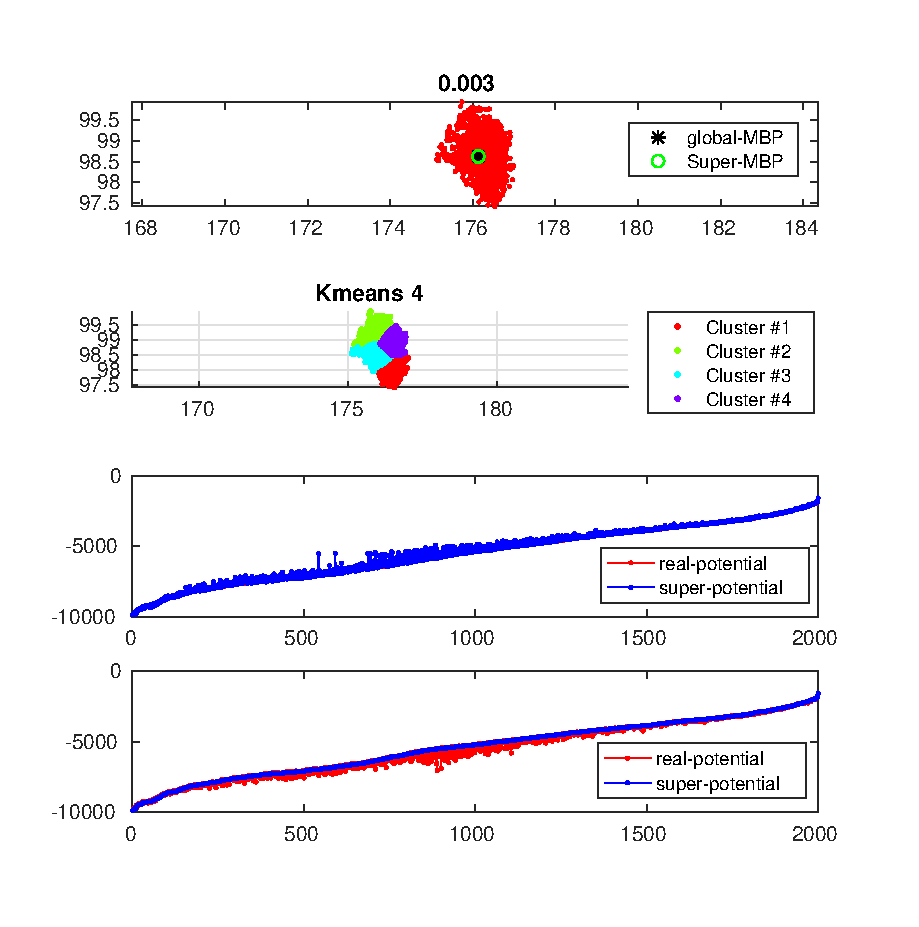
\includegraphics[scale=0.45]{sp_p_mixed_kmeans}
\end{subfigure}%
~ 
\begin{subfigure}[t]{0.5\textwidth}
\centering
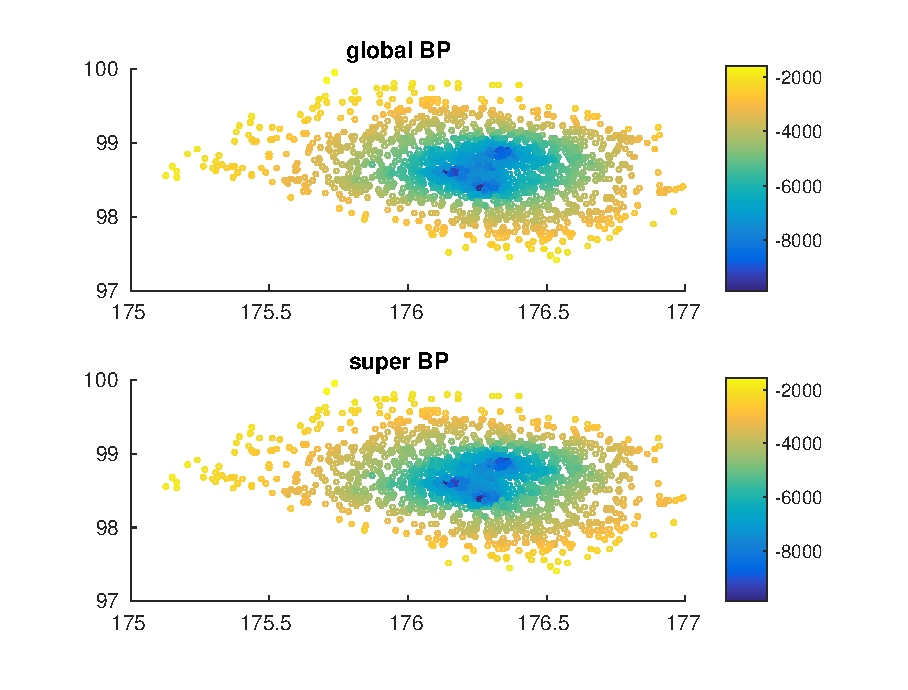
\includegraphics[scale=0.45]{sp_p_mixed_kmeans_bp}
\end{subfigure}
\caption{Result of Algorithm \ref{sp-mixed}}
\end{figure*}

 \begin{algorithm}
\caption{Super-particle Hierarchy}
\label{sp-p}
\begin{algorithmic}[1]
\Procedure {$MBP=sp_kmeans(X,m)$}{}
\State $[IDX,c]=kmeans(X,N_c)$ 
\State $\bar m_i=|\{j | IDX(j)=i\}|,\,\forall i=1:N_c$
\State $MBP=\ds\min_i \ds\sum_{\{j|IDX(i)\neq j\}}\frac{\bar m_j}{d(X_i,c_j)}$ 
\State $n_c=N_c$
\State $k=1$
\While{$k\leq n_k$}
\State $MBP_{old} = MBP$
\State $v=\{j\,|\,IDX(j)=IDX(MBP)\}$
\State $[\tilde{IDX},\tilde{c}]=kmeans(X(i),\tilde{N_c}$
\State $c=\{c_1,\dots,c_{MBP-1}\}\cup\tilde{c}_1 \cup \{c_{MBP+1},\dots,c_{N_c}\}\cup \{\tilde{c}_2,\dots,\tilde{c}_{\tilde{N_c}}\}\}$
\State $IDX(v)=\tilde{IDX}+kN_c-1$
\State $n_c=n_c-1+\tilde{N_c}$
\State $\bar m_i=\frac{1}{|\{j | IDX(j)=i\}|},\,\forall i=1:n_c$
\State $MBP=\ds\min_i \ds\sum_{\{j|IDX(i)\neq j\}}\frac{\bar m_j}{d(X_i,c_j)}$ 
\If{$MBP=MBP_{old}$}
\State Stop
\EndIf
\State $k=k+1$
\EndWhile
\EndProcedure
\end{algorithmic} 
 \end{algorithm}
\begin{figure*}[t!]
\centering
\begin{subfigure}[t]{0.5\textwidth}
\centering
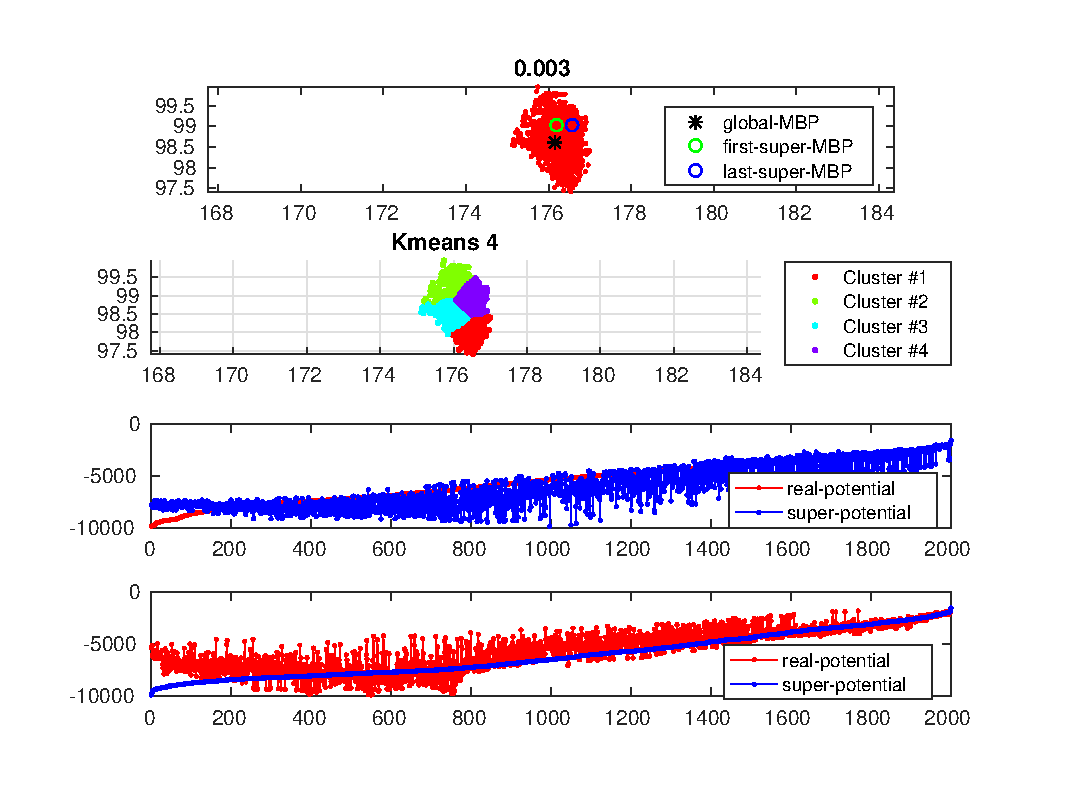
\includegraphics[scale=0.45]{sp_p_kmeans}
\end{subfigure}%
~ 
\begin{subfigure}[t]{0.5\textwidth}
\centering
\includegraphics[scale=0.45]{sp_p_kmeans_bp}
\end{subfigure}
\caption{Result of Algorithm \ref{sp-p}}
\end{figure*}
\begin{figure}[h]
\centering
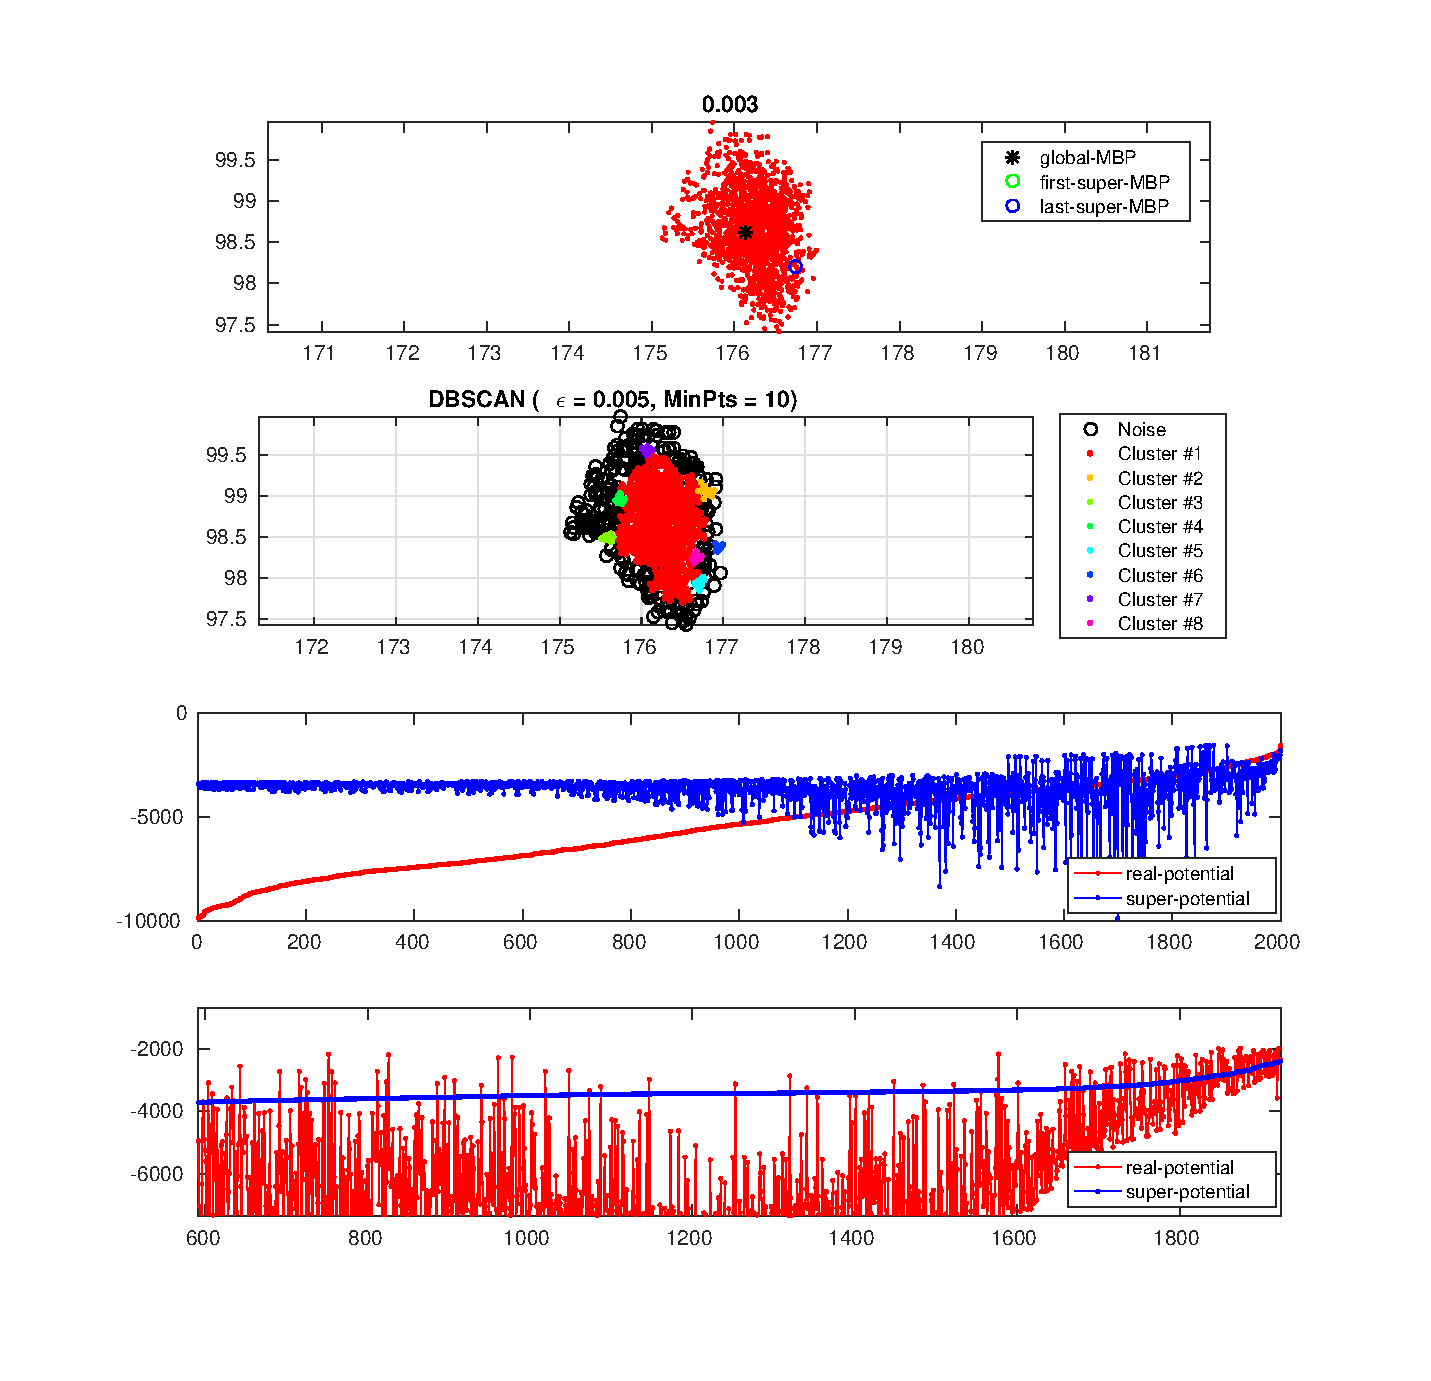
\includegraphics[scale=0.45]{sp_p_dbscan}%
\caption{Result of replacing Kmeans by DBSCAN in Algorithm \ref{sp-p}}
\label{fig:sp_dbscan}
\end{figure}

 \begin{algorithm}
\caption{Locate MBP from a subset of particles which forms the most dense super-particle via DBSCAN}
\label{dbscan_max}
\begin{algorithmic}[1]
\Procedure {$MBP=mbp_dbscan_max(X,m)$}{}
\State $[IDX,c]=dbscan(X,\varepsilon)$, where $\varepsilon$ is the linkage length provided for DBSCAN. 
\State $\bar m_i=|\{j | IDX(j)=i\}|,\,\forall i=1:N_c$, where $N_c$ is the resulted number of clusters given $\varepsilon$
\State $i_s=\ds\max_i \bar{m_i}$
\State $V=\{j \,|\, IDX(j)=i_s\}$
\State $SBP_i=\ds\sum_{\{j|IDX(i)\neq j\}}\frac{\bar m_j}{d(X_i,c_j)}+\ds\sum_{\{j|IDX(j)=IDX(i),i\neq j\}}\frac{m_j}{d(X_i,X_j)},\, \forall i\in V$ 
\State $MBP=\ds\min_{i\in V} SBP_i$
\EndProcedure
\end{algorithmic} 
 \end{algorithm}
\begin{figure}[H]
\centering
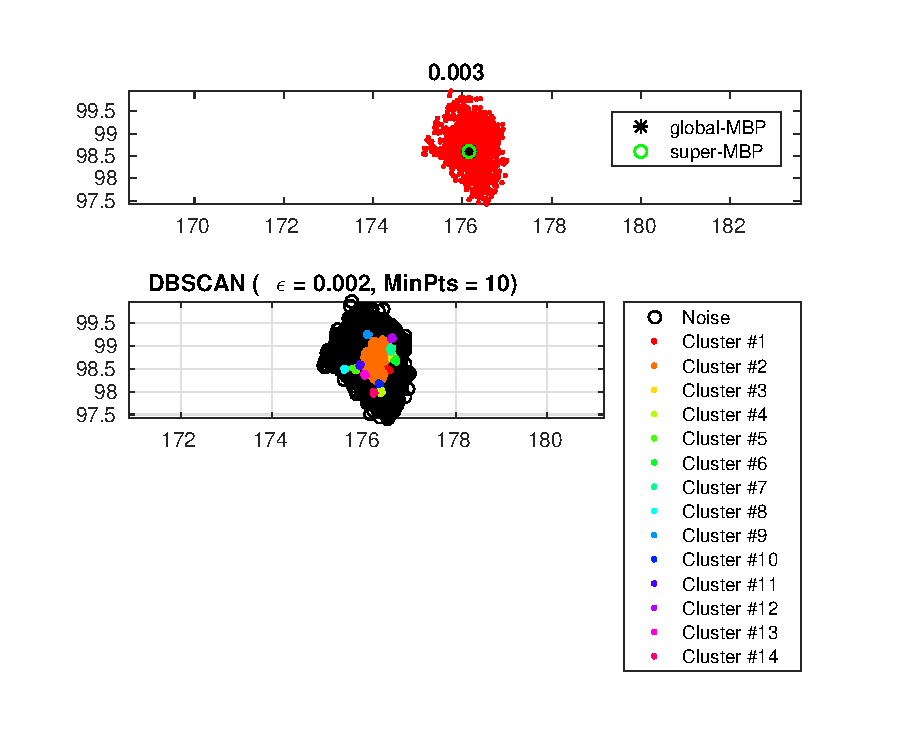
\includegraphics[scale=0.45]{p_dbscan_maxSub}%
\caption{Result of Algorithm \ref{dbscan_max}}
\label{fig:dbscan_max}
\end{figure}
\end{document}

